\section[Defining the signature]{Defining the \signature{}}
\label{sec:defHomotopy}

\begin{figure}
    \centering
    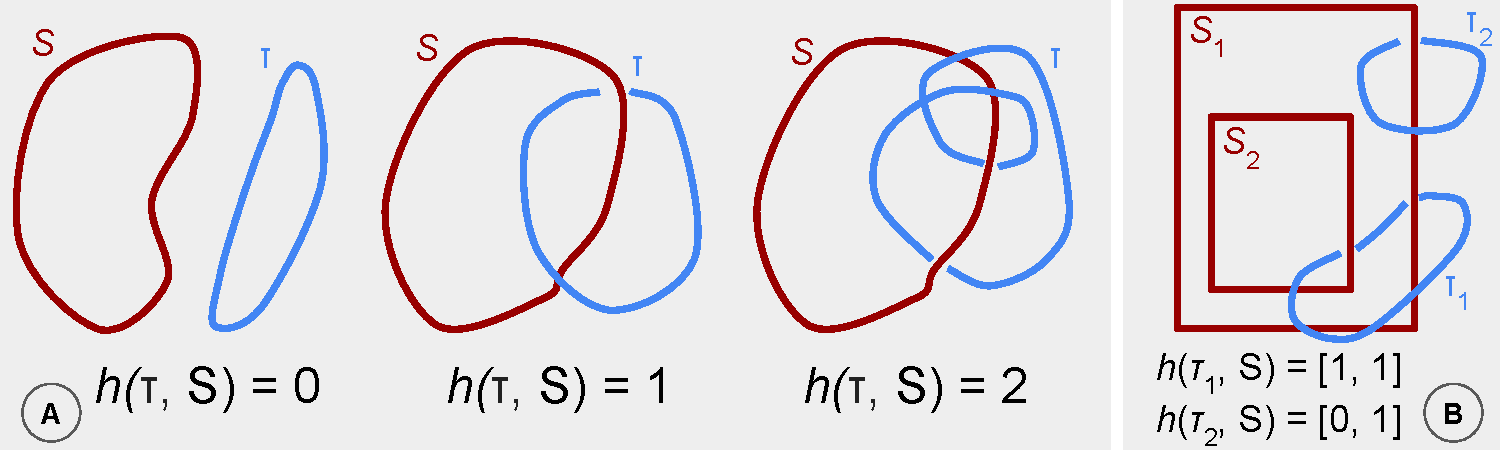
\includegraphics[width=\linewidth]{Chap5/images/simple_h.pdf}
    \caption{(A) Illustration of the h-signature for a loop representing the robot and DOO (blue) and a loop representing an obstacle (solid red). (B) Two examples of the h-signature for a skeleton with two obstacle loops $S_1$ and $S_2$.}
    \label{fig:simple_h}
\end{figure}

\subsection{Preliminaries}

We primarily use notation that is consistent with \cite{Bhattacharya11}. We call a closed one-dimensional curve in 3D a \textit{loop}. The environment is assumed to be decomposed into a \textit{skeleton} made up of multiple \textit{obstacle loops} $\skels = \{\skel_1,\dots,\skel_n\}$. Each obstacle loop is made up of line segments $\skel_i=\{\textbf{s}_i^1,\dots,\textbf{s}_i^{n_i}\}$. An example environment and corresponding skeleton is shown in Figure \ref{fig:constructingSignature}. In practice, the skeleton can either be specified manually or computed automatically from a medial axis transform of a mesh or pointcloud of the environment.

\cite{Bhattacharya11} plans paths that are in a given homotopy class or avoid a certain homotopy class. They compare two paths by considering the homotopy class of the closed loop $\tau$ formed by joining the two paths at their shared start and end points. For a path loop $\tau$ and an obstacle loop $\skel$, \cite{Bhattacharya11} defines the h-signature $h(\tau, \skel) \in \mathbb{Z}$, which counts the number of times $\tau$ passes through $\skel$. The sign of $h$ in this case is determined by the direction of $\tau$. The h-signature can be extended to a list of the h-signatures with respect to each obstacle loop in the skeleton $h(\tau, \skels)) = [h(\tau,\skel_1), \dots,h(\tau,\skel_n)]$. These cases are illustrated in Figure \ref{fig:simple_h}. The equation for computing $h(\tau,\skel)$ is reproduced from \cite{Bhattacharya11}. The point $\sk_i^{j'}$ is the point that follows $\sk_i^j$, and $r$ is a point on the loop $\tau$. The integration over $\tau$ is done numerically.

\begin{equation}
\label{eq:hsig}
\begin{split}
    h(\tau,\skel) = \frac{1}{4\pi} \int_{\tau}\sum_{j=1}^{n_i}\Phi(\sk_i^j,\sk_i^{j'}, r) \Delta r \\
    \Phi(\sk_i^j,\sk_i^{j'}, r) = \frac{1}{||d||^2} \Big( \frac{d\times p'}{||p'||} - \frac{d \times p}{||p||} \Big) \\
    p=\sk_i^j-r,\quad p'=\sk_i^{j'},\quad d=\frac{(\sk_i^{j'}-\sk_i^j)\times(p\times p')}{||\sk_i^{j'} - \sk_i^j||^2}
\end{split}
\end{equation}

We take this idea but apply it to grasp loops, instead of paths. Unlike in path planning, where the direction of $\tau$ matters, we only care how or whether loops are linked. Accordingly, we assert that $h$ is always non-negative.

\subsection[Computing the signature]{Computing the \signature{}}

\begin{figure}
    \centering
    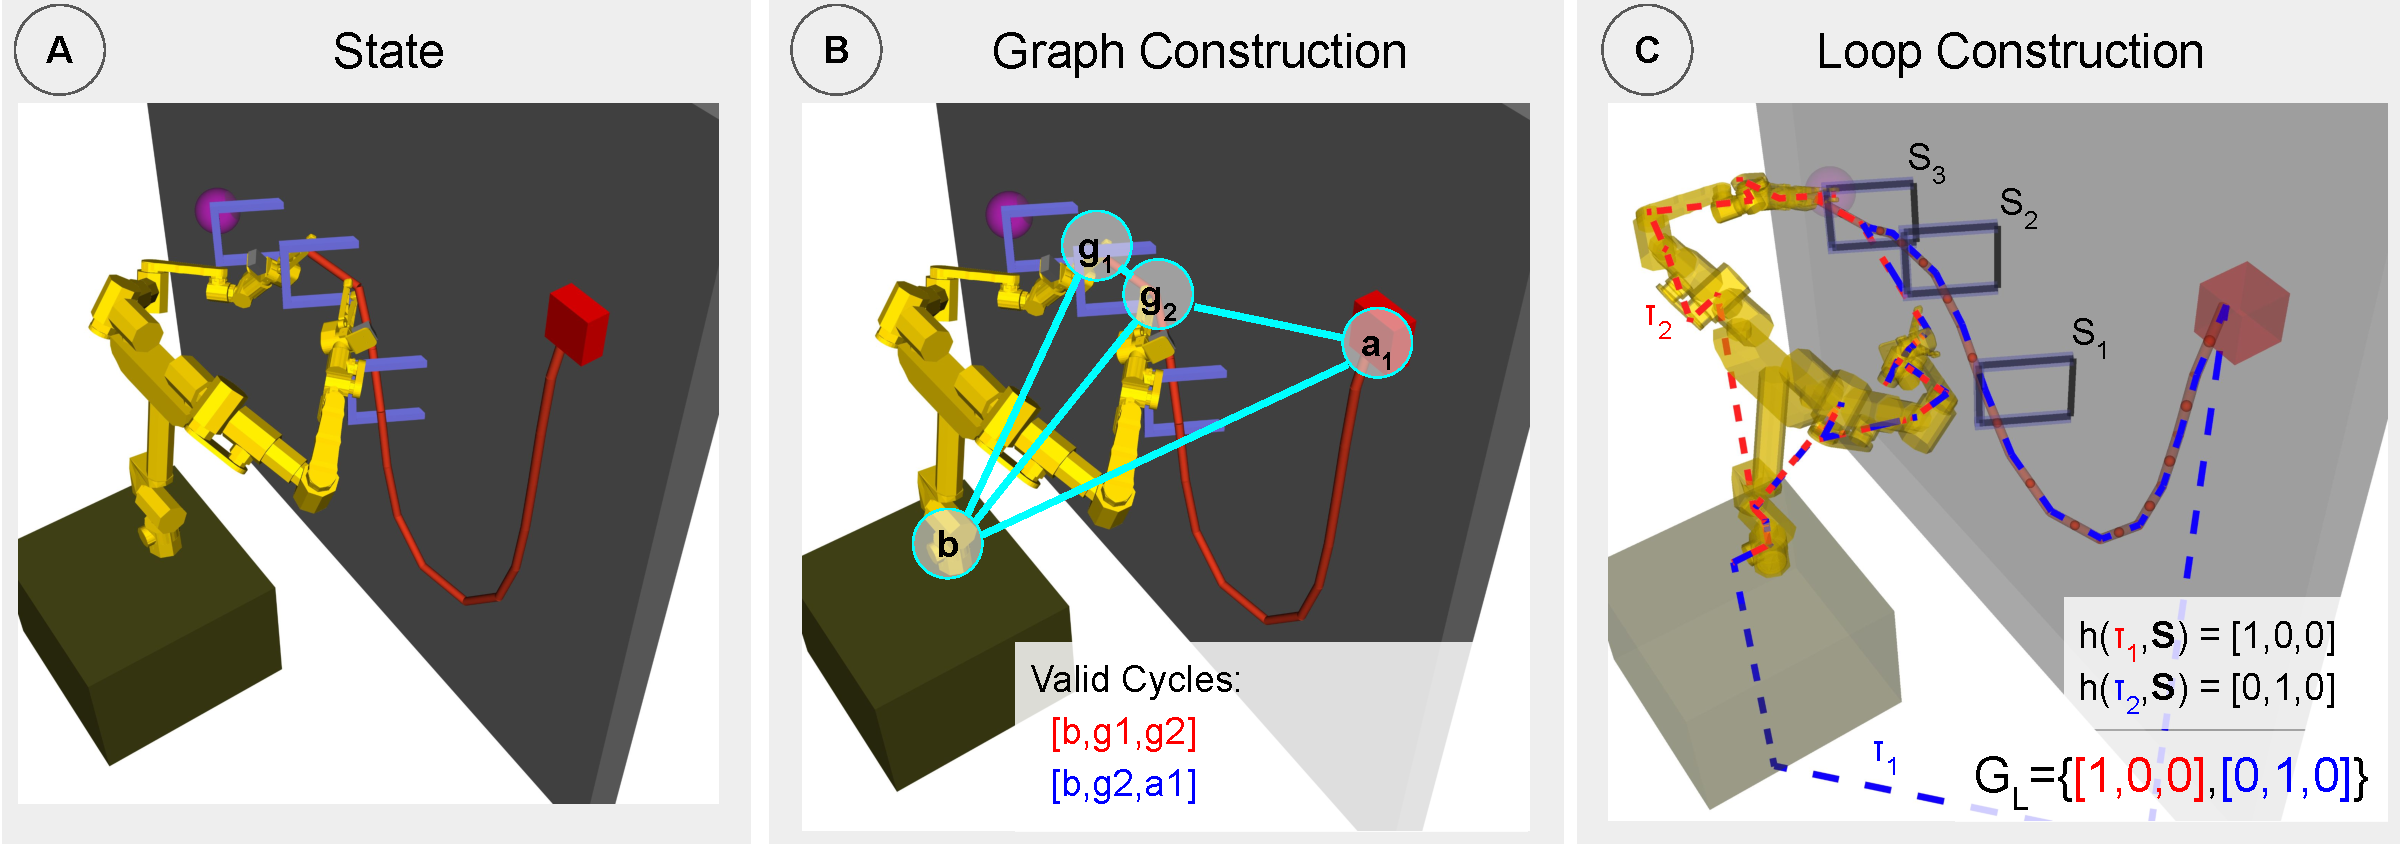
\includegraphics[width=\linewidth]{Chap5/images/alg.pdf}
    \caption{The process of constructing the \signature{}. (C) There are 2 grasp loops and 3 object loops, so the \signature{} is a set with two elements, and each element is a vector of 3 non-negative integers.}
    \label{fig:constructingSignature}
\end{figure}

The \signature{} is composed of the h-signatures $h(\tau, \skels)$ of grasp loops $\tau$ formed by the robot and  DOO. We describe the process here and in Algorithm \ref{chap5:alg:computing_signature}. The grasp loops are constructed based on a graphical model of the state $\mathcal{G}=(V,E)$ where vertices are the robot base, its grippers, and attach points, and edges are paths between them. Attach points are used to represent locations on the DOO which are fixed relative to the robot (e.g plugged into the wall or rigidly mounted on the robot itself). Figure \ref{fig:constructingSignature} illustrates how the graph construction step works. The robot base vertex is connected to all gripper and attach vertices because it connects to the grippers directly (via the robot geometry) and the attach points indirectly (via the environment). Edges connect grippers/attach points to one another if they are adjacent on the DOO. In Figure \ref{fig:constructingSignature}, the vertices $(g_1,g_2)$ are adjacent, as are $(g_2,a_1)$, but $(g_1,a_1)$ are not. In Algorithm \ref{chap5:alg:addEdges}, the function $\Adj(v_i,v_j,\state)$ checks for adjacency between $v_i$ and $v_j$ at the given state $\state$.

From $\mathcal{G}$, we extract all cycles $\cycles$ of exactly 3 distinct vertices which contain a gripper (\getValidCycles), and convert each cycle to a grasp loop $\tau$ (\getLoops). To make a grasp loop from a cycle, we concatenate the 3D paths represented by the cycles' edges. This requires a skeletonized representation of the robot geometry, which can be constructed from the kinematic tree and the origins of the links, as well as the points representing the DOO. A path between the robot base and an attach point (e.g. $(b,a_1)$ in Figure \ref{fig:constructingSignature}) can be chosen arbitrarily, as long as it is the same for all states. Cycles not containing a gripper (e.g. $(b,a_1,a_2)$) are omitted for compactness, since attach points presumably cannot be changed by the planner.

For each grasp loop, we compute the associated h-signature $h(\tau_i, \skels)$. The \signature{} of the state, denoted $\sig(\state)$, is the \textit{multiset} of the h-signatures of each grasp loop. In a multiset the order does not matter, but elements may repeat. The number of repetitions of an element is called its multiplicity. Two multisets are equivalent if their elements and multiplicities are equal. Preserving repetitions in the \signature{} allows us to represent multiple grasp loops that go through the same obstacle loop.

This may result in a grasp loop containing two grippers that has $h(\tau,\skels)=\bm{0}$ (i.e. not linked $\skels$). The red dashed grasp loop shown in Figure \ref{fig:examples} B3 is an example of this. Releasing one of the grippers does not categorically change what we can do with the object, and neither would grasping with an additional gripper right next to two already grasping. Therefore, if there is a cycle with $h(\tau,\skels)=\bm{0}$ containing two grippers, one of the grippers is removed from the graph and the process restarts from the graph construction step (Lines 7-16 in \ref{chap5:alg:computing_signature}).

This graph construction assumes a fixed base, but by constructing the graph differently, we can adapt to other scenarios. For example, we might connect drones flying together in a swarm, even though there may not be a physical connection between them. Two drones grasping the DOO simultaneously would form a loop (Fig \ref{fig:examples} E), allowing us to plan over the scene's topology.

\begin{algorithm}[t]
    \caption{Compute the \signature{}}\label{chap5:alg:computing_signature}
    \SetAlgoLined
    \DontPrintSemicolon
    \SetKwInOut{Input}{Input}
    \SetKwInOut{Output}{Output}
    
    \Input{$V, \skels, \state$}
    \Output{$\sig(\state)$}
    
   $\mathcal{G} = \addEdges(V, \state)$ \tcp*{Graph construction}
   $\cycles = \getValidCycles(\mathcal{G})$ \\
   \If{$|\cycles| = 0$}{
      \Return{$\emptyset$} \\
   }
   $\tau = \getLoops(\mathcal{G},\cycles,\state)$ \\
   \tcp{Remove empty gripper-gripper cycles (optional)}
   \For{$\tau_i \in \tau, o_i \in \cycles$}{
      \If{$h(\tau_i, \skels) = 0$}{
         \For{$v_i, v_j \in o_i$}{
            \If{$v_i,v_j$ \texttt{are gripper vertices}}{
               $V = V \setminus v_j$ \tcp*{choice of $v_j$ or $v_i$ is arbitrary}
               \textbf{goto 1} \texttt{Graph construction} \\
            }
         }
      }
   }
   \tcp{Compute final \signature{}}
   $\sig(\state) = \texttt{MultiSet}\{h(\tau_i, \skels) | \tau_i \in \tau\}$ \\
   \Return{$\sig(\state)$}
\end{algorithm}

\begin{algorithm}
    \caption{\addEdges}\label{chap5:alg:addEdges}
    \SetAlgoLined
    \DontPrintSemicolon
    \SetKwInOut{Input}{Input}
    \SetKwInOut{Output}{Output}
    
    \Input{$V, \state$}
    \Output{$\mathcal{G}$}
    
    $E = \emptyset$ \\
    \For{$v_i \in V$}{
        \For{$v_j \in V$}{
            \tcp{Skip invlid edges}
            \If{$v_i = v_j$}{
                \texttt{continue}
            }
            \ElseIf{$\neg\Adj(v_i,v_j,\state)$}{
                \texttt{continue}
            }
            $E = E \cup (v_i,v_j)$ \tcp*{Add the edge}
        }
    }
    \Return{$E$}
\end{algorithm}

\subsection{Computational Complexity}

The complexity of computing the \signature{} can be written in Big-O notation based on the number of skeletons $n_s$, number of line segments in the skeleton $l_s$, arms and/or attach points $n_a$, and the length of the arms and/or DOO $l_a$. In the base case of $n_a=2$, the graph has 3 vertices and at most cycle of length 3. And adding another vertex adds at most one cycle, so in the worst case $n_a$ arms/attach points create $n_a-1$ loops. Each cycle (loop) is compared with each skeleton, and the number of comparisons scales linearly with both the number of line segments and the length of the loop, giving a total complexity of $O\big((n_a-1) n_s l_s l_a\big)$. Our Python implementation using the NetworkX library \cite{NetworkX} for computing the \signature{} for a state takes $\leq$10ms in all environments.